\documentclass[10pt, english, fleqn, DIV=15, headinclude]{scrartcl}

\usepackage[bibatend, color]{header}

\hypersetup{
    pdftitle=
}

\ihead{English panels for laundy appliances in FZ Jülich Guest house}
\ohead{Page \thepage}
\cfoot{}

%\subject{}
\title{}
%\subtitle{}
\author{
    Martin Ueding \\ \small{\href{mailto:mu@martin-ueding.de}{mu@martin-ueding.de}}
}

\begin{document}

\section*{Washing machines}

If you have no idea what to do, “easy-care” with \SI{40}{\celsius}
\emph{should} be fine for most clothes. Read the tags in your clothes to be
sure as I am not responsible for your actions!

\subsection*{Siemens}
\includegraphics[width=\linewidth]{Washing-Siemens-1.pdf}

\subsection*{AEG}
\includegraphics[width=\linewidth]{Washing-AEG-1.pdf}

\subsection*{Zanussi}
\includegraphics[width=\linewidth]{Washing-Zanussi-1.pdf}

\subsection*{Miele}
\includegraphics[width=\linewidth]{Washing-Miele-1.pdf}

\subsection*{Detergent drawer}


\includegraphics[width=.3\linewidth]{Detergent.pdf}


\section*{Drying machines}

\subsection*{Miele 1}

\includegraphics[width=\linewidth]{Dryer-Miele-1.pdf}

\subsection*{Miele 2}

\includegraphics[width=\linewidth]{Dryer-Miele-2.pdf}

\vfill

\begin{small}
    Made by Martin Ueding (mu@martin-ueding.de) in 2015. If you want the PDF or
    contribute to this document, just email me. You may redistribute this
    document under the \emph{Creative Commons Attribution 4.0 International}
    (CC-BY) license.
    This document is neither affiliated to the FZ Jülich or the guest house
    management.
    Although I created this with care and best intentions, I do not take any
    form of liability or responsibility for any damage, e.g. interpreting this
    incorrectly and damaging laundry. Use it on your own risk!
\end{small}

\end{document}

% vim: spell spelllang=en tw=79
